%%%%%%%%%%%%%%%%%%%%%%%%%%%%%%%%%%%%%%%%%%%%%%%%%%%%%%%%%%
% This compiles both the English IPA consonant and vowel %
% charts (_consonants and _vowels) into an actual        %
% document.                                              %
%                                                        %
% Compile with XeLaTeX                                   %
%                                                        %
% -Joshua McNeill (joshua dot mcneill at uga dot edu)    %
%%%%%%%%%%%%%%%%%%%%%%%%%%%%%%%%%%%%%%%%%%%%%%%%%%%%%%%%%%

\documentclass{article}
  % Read in standard preamble (cosmetic stuff)
  %%%%%%%%%%%%%%%%%%%%%%%%%%%%%%%%%%%%%%%%%%%%%%%%%%%%%%%%%%%%%%%%
% This is a standard preamble used in for all materials        %
% documents. It basically contains cosmetic settings.          %
%                                                              %
% Joshua McNeill                                               %
% joshua dot mcneill at uga dot edu                            %
%%%%%%%%%%%%%%%%%%%%%%%%%%%%%%%%%%%%%%%%%%%%%%%%%%%%%%%%%%%%%%%%

% Packages and settings
\usepackage{fontspec}
  \setmainfont{Charis SIL}
\usepackage{hyperref}
  \hypersetup{colorlinks=true,
              allcolors=blue}


  % Packages and settings
  \usepackage{adjustbox}
  \usepackage{tikz}
  \usepackage{hyperref}
    \hypersetup{colorlinks=true,
                allcolors=blue}

  % Document information
  \title{Empty IPA charts}
  \date{}

  %% Custom commands
  % Space between heading and chart
  \newcommand{\headspace}{0.4cm}

\begin{document}
  \maketitle
  CONSONANTS

  \vspace{\headspace}

  \begin{adjustbox}{width=\textwidth}
    % Read in the consonants IPA chart
    %%%%%%%%%%%%%%%%%%%%%%%%%%%%%%%%%%%%%%%%%%%%%%%%%%%%%%%%%%
% This creates an English IPA chart for consonants       %
%                                                        %
% Compiled from material_IPA_en_chart.tex when a         %
% standalone document is needed                          %
%                                                        %
% -Joshua McNeill (joshua dot mcneill at uga dot edu)    %
%%%%%%%%%%%%%%%%%%%%%%%%%%%%%%%%%%%%%%%%%%%%%%%%%%%%%%%%%%

\begin{tabular}{| l | c c | c c | c c | c c | c c | c c | c c | c c | c c | c c | c c |}
  \hline
  & \multicolumn{2}{c}{Bilabial} & \multicolumn{2}{c}{Labiodental} & \multicolumn{2}{c}{Dental} & \multicolumn{2}{c}{Alveolar} & \multicolumn{2}{c}{Postalveolar} & \multicolumn{2}{c}{Retroflex} & \multicolumn{2}{c}{Palatal} & \multicolumn{2}{c}{Velar} & \multicolumn{2}{c}{Uvular} & \multicolumn{2}{c}{Pharyngeal} & \multicolumn{2}{c}{Glottal} \\
  \hline
  Plosive/Stop &   &   &   &   &   &   &   &   &   &   & & & &   &   &   & & & & &   & \\
  \hline
  Nasal        &   &   &   &   &   &   &   &   &   &   & & & &   &   &   & & & & &   & \\
  \hline
  Trill        &   &   &   &   &   &   &   &   &   &   & & & &   &   &   & & & & &   & \\
  \hline
  Tap/Flap     &   &   &   &   &   &   &   &   &   &   & & & &   &   &   & & & & &   & \\
  \hline
  Fricative    &   &   &   &   &   &   &   &   &   &   & & & &   &   &   & & & & &   & \\
  \hline
  \begin{tabular}{@{} l @{}}
    Lateral \\
    fricative
  \end{tabular}&   &   &   &   &   &   &   &   &   &   & & & &   &   &   & & & & &   & \\
  \hline
  Approximant  &   &   &   &   &   &   &   &   &   &   & & & &   &   &   & & & & &   & \\
  \hline
  \begin{tabular}{@{} l @{}}
    Lateral\\
    approximant
  \end{tabular}&   &   &   &   &   &   &   &   &   &   & & & &   &   &   & & & & &   & \\
  \hline
\end{tabular}

  \end{adjustbox}

  {\tiny *Symbols on the right side of a box represent voiced sounds and on the left voiceless sounds.}

  \vspace{2cm}

  \parbox[l]{0.5\textwidth}{
    OTHER SYMBOLS

    \vspace{\headspace}

    \begin{adjustbox}{width=0.4\textwidth}
      \begin{tabular}{c l}
           & Voiced labial-velar approximant \\
           & Voiceless affricate \\
           & Voiced affricate
      \end{tabular}
    \end{adjustbox}
  }
  \parbox[r]{0.5\textwidth}{
    VOWELS

    \vspace{\headspace}

    \begin{adjustbox}{width=0.4\textwidth}
      % Read in the vowels IPA chart
      %%%%%%%%%%%%%%%%%%%%%%%%%%%%%%%%%%%%%%%%%%%%%%%%%%%%%%%%%%%%%%%%%%%%%%%%%%%%%%%%%%%%%
% This creates an English IPA chart for vowels                                      %
%                                                                                   %
% Compiled from material_IPA_en_chart.tex when a                                    %
% standalone document is needed                                                     %
%                                                                                   %
% Code is only slightly from:                                                       %
%   https://tex.stackexchange.com/questions/156955/tikz-pgf-linguistics-vowel-chart %
%                                                                                   %
% -Joshua McNeill (joshua dot mcneill at uga dot edu)                               %
%%%%%%%%%%%%%%%%%%%%%%%%%%%%%%%%%%%%%%%%%%%%%%%%%%%%%%%%%%%%%%%%%%%%%%%%%%%%%%%%%%%%%

% Custom command
\def\V(#1,#2){barycentric cs:hf={(3-#1)*(2-#2)},hb={(3-#1)*#2},lf={#1*(2-#2)},lb={#1*#2}}

% Chart
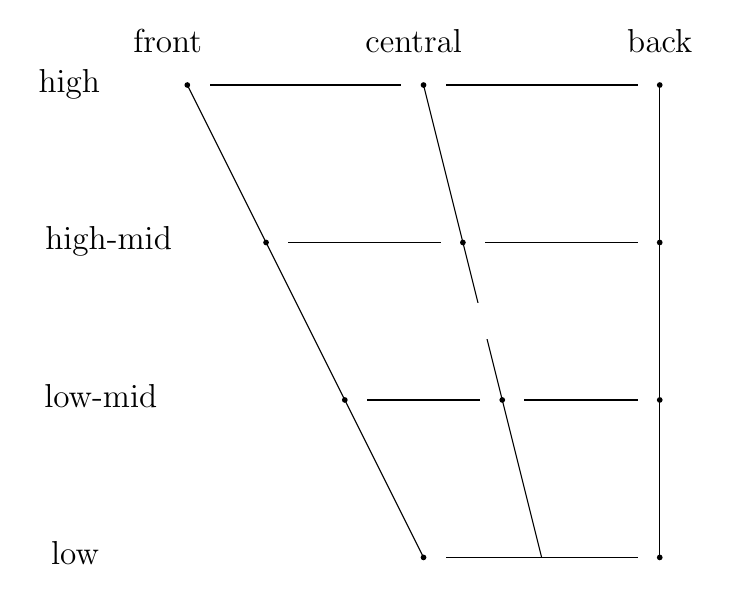
\begin{tikzpicture}[scale=3]
  \large
  \tikzset{
    vowel/.style={fill=white, anchor=mid, text depth=0ex, text height=1ex},
    dot/.style={circle,fill=black,minimum size=0.4ex,inner sep=0pt,outer sep=-1pt},
  }
  \coordinate (hf) at (0,2); % high front
  \coordinate (hb) at (2,2); % high back
  \coordinate (lf) at (1,0); % low front
  \coordinate (lb) at (2,0); % low back
  \def\V(#1,#2){barycentric cs:hf={(3-#1)*(2-#2)},hb={(3-#1)*#2},lf={#1*(2-#2)},lb={#1*#2}}

  % Draw the horizontal lines first.
  \draw (\V(0,0)) -- (\V(0,2));
  \draw (\V(1,0)) -- (\V(1,2));
  \draw (\V(2,0)) -- (\V(2,2));
  \draw (\V(3,0)) -- (\V(3,2));

  % Place all the unrounded-rounded pairs next, on top of the horizontal lines.
  \path (\V(0,0))     node[vowel, left] { } node[vowel, right] { } node[dot] {};
  \path (\V(0,1))     node[vowel, left] { } node[vowel, right] { } node[dot] {};
  \path (\V(0,2))     node[vowel, left] { } node[vowel, right] { } node[dot] {};
  \path (\V(0.5,0.4)) node[vowel, left] { } node[vowel, right] { } node[   ] {};
  \path (\V(0.5,1.6)) node[vowel, left] { } node[vowel, right] { } node[   ] {};
  \path (\V(1,0))     node[vowel, left] { } node[vowel, right] { } node[dot] {};
  \path (\V(1,1))     node[vowel, left] { } node[vowel, right] { } node[dot] {};
  \path (\V(1,2))     node[vowel, left] { } node[vowel, right] { } node[dot] {};
  \path (\V(2,0))     node[vowel, left] { } node[vowel, right] { } node[dot] {};
  \path (\V(2,1))     node[vowel, left] { } node[vowel, right] { } node[dot] {};
  \path (\V(2,2))     node[vowel, left] { } node[vowel, right] { } node[dot] {};
  \path (\V(2.5,0))   node[vowel, left] { } node[vowel, right] { } node[   ] {};
  \path (\V(3,0))     node[vowel, left] { } node[vowel, right] { } node[dot] {};
  \path (\V(3,2))     node[vowel, left] { } node[vowel, right] { } node[dot] {};

  % Draw the vertical lines.
  \draw (\V(0,0)) -- (\V(3,0));
  \draw (\V(0,1)) -- (\V(3,1));
  \draw (\V(0,2)) -- (\V(3,2));

  % Place the unpaired symbols last, on top of the vertical lines.
  \path (\V(1.5,1))   node[vowel]       { };
  \path (\V(-0.25,0)) node[vowel]       {front};
  \path (\V(-0.25,1)) node[vowel]       {central};
  \path (\V(-0.25,2)) node[vowel]       {back};
  \path (\V(0,-0.5))  node[vowel]       {high};
  \path (\V(1,-0.8))  node[vowel]       {high-mid};
  \path (\V(2,-1.55)) node[vowel]       {low-mid};
  \path (\V(3,-2.95)) node[vowel]       {low};
\end{tikzpicture}

    \end{adjustbox}
  }

  \begin{flushright}
    {\tiny
      Symbols on the right side of a node represent rounded vowels and on the left unrounded.

      ``High'' is synonymous with ``close''.

      ``Low'' is synonymous with ``open''.

      Bold vowels are lax, the rest are tense.

      {[} ] is a mid central unrounded vowel.
    }
  \end{flushright}
\end{document}
